\begin{figure}[ht!]
%
% \begin{center}
% \centering
\begin{subfigure}[t]{0.23\textwidth}
% \centering
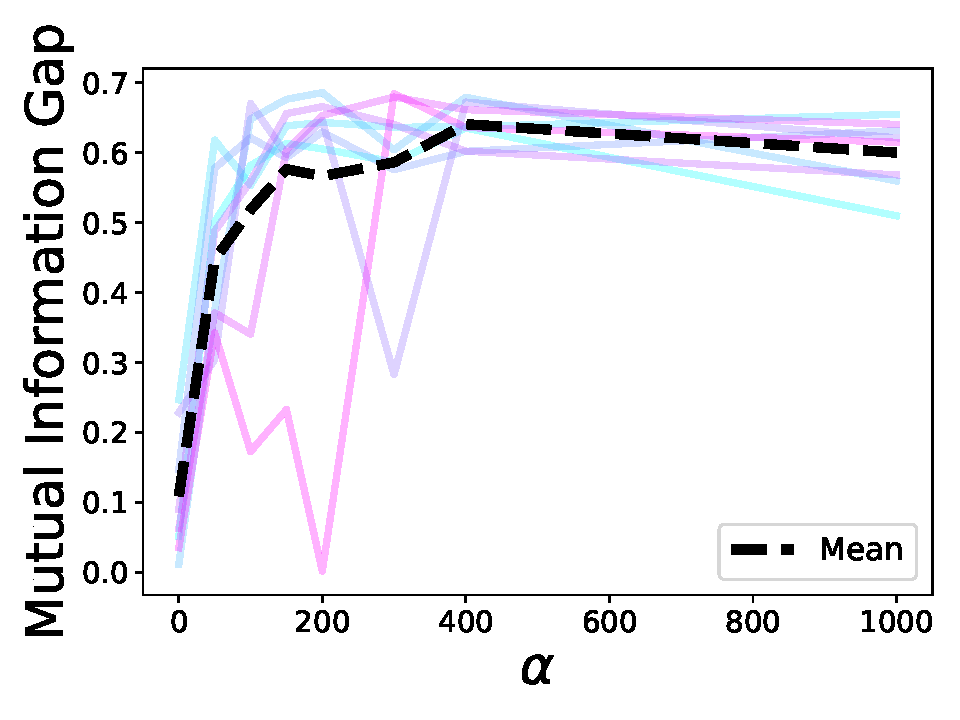
\includegraphics[width=\textwidth]{mig_beta_sens_gamma_lines.pdf}
\caption{Color is $\gamma$, brighter colours $\longrightarrow$ higher values}
\label{fig:dsprites-mig-lines}
\end{subfigure}
%
\hfill
%
\begin{subfigure}[t]{0.23\textwidth}
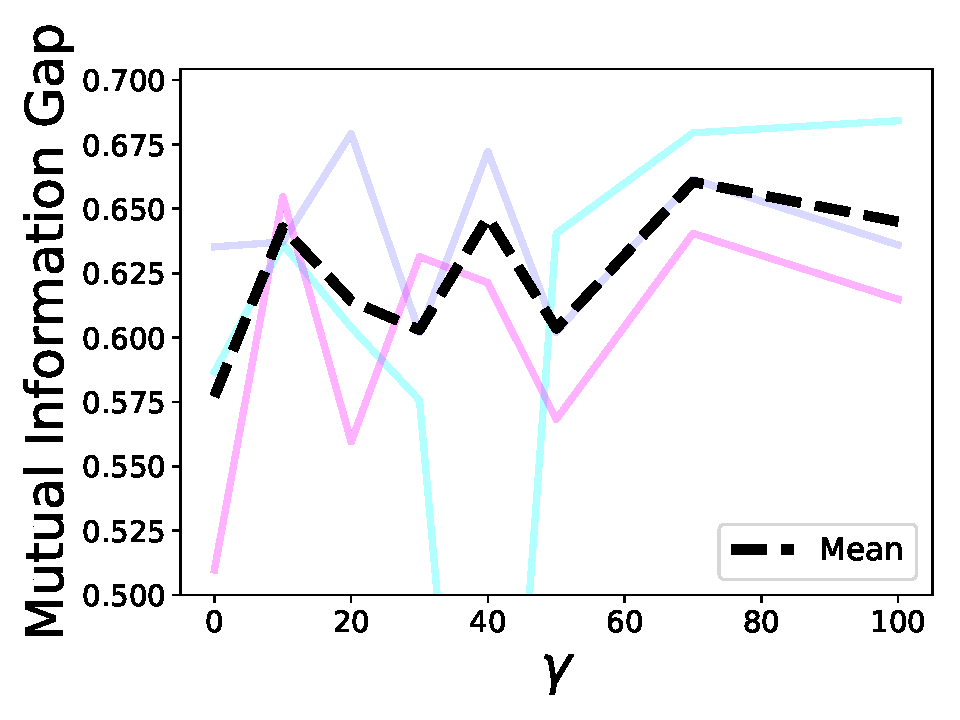
\includegraphics[width=\textwidth]{mig_gamma_beta_sens_high_lines.pdf}
\caption{Colour is $\alpha$, brighter colors $\longrightarrow$ higher values}
\label{fig:dsprites-mig-lines-high-alpha}
\end{subfigure}


\caption{
    Mutual Information Gap (MIG) for various $(\alpha, \gamma)$ settings of the FFVAE. 
    In Fig. \ref{fig:dsprites-mig-lines}, each line is a different value of
    $\gamma \in [10, 20, 30, 40, 50, 70, 100]$, with brighter colors indicating larger values of $\gamma$.
    In Fig. \ref{fig:dsprites-mig-lines-high-alpha}, each line is a different value of
    $\alpha \in [300, 400, 1000]$, with brighter colors indicating larger values of $\alpha$.
    Models trained on DspritesUnfair, MIG calculated on Dsprites.
    Higher MIG is better.
    Black dashed line indicates mean (with outliers excluded).
    $\alpha = 0$ is equivalent to the FactorVAE.
    }
    \label{fig:dsprites-mig}
% \end{center}
% \vskip -0.2in
\end{figure}

